% !TeX root = ../main.tex
% !TeX root = ../main.tex
% Add the above to each chapter to make compiling the PDF easier in some editors.

\chapter{Scaling TUM-Live}\label{chapter:scaling_tumlive}

This chapter focuses on applying the concepts discussed in the previous sections to the architecture of TUM-Live, discussing the development approach, results and challenges along the way. 

\section{Process, Preparation, Methods and Environments}

The thesis spanned 5 months, from 15.05.2024 to \getSubmissionDate{}. The first weeks were spent familiarizing with the current system considering different approaches to scale its architecture and finding potential bottlenecks or issues. Following the initial analysis of the system, before being able to try scaling individual components, the original user and role system first needed to be updated together with new database models. After that, the most important components were gradually updated to be usable and manageable by different organizations. 
To develop and test the prototype of a distributed architecture for TUM-Live for this thesis, the following resources were used:
\begin{itemize}
    \item 3 \ac{VM}s with: 2 GB RAM, Intel(R) Xeon(R) CPU E5-2697A v4 @ 2.60GHz
    \item 1 \ac{VM} with: 20 GB RAM, AMD EPYC 7452 32-Core Processor
    \item 1 \ac{AWS} \ac{EKS} Cluster
    \item 1 selfhosted \ac{VM} with 32 GB RAM, AMD Ryzen 7 PRO 6850U @ 2.70GHz
\end{itemize}

\noindent After the target architecture had been deployed (on a smaller scale) using given resources, a set of performance tests and comparisons was made to find potential limits and breakpoints of each component. 
Additionally, in parallel to the development of the new architecture, a dedicated documentation has been created to facilitate the setup of GoCast for lecturers or new schools, which can be found at \href{https://tumlive-docs.pages.dev/}{tumlive-docs.pages.dev}. The documentation was created using Meta Opensource's \href{https://github.com/facebook/docusaurus}{Docusaurus}\footnote{\url{https://github.com/facebook/docusaurus}}. Static pages were deployed using Cloudflare.
All relevant source code for the thesis, new architecture, other mentioned prototypes and documentation can also be found at \href{https://github.com/carlobortolan/thesis}{github.com/carlobortolan/thesis}.

\section{Proposed System}

As explained in \autoref{section:tum-live-history}, to use TUM-Live, currently, each lecture hall needs to be equipped with a \ac{SMP} device, which can cost up to 10,000 EUR. With the creation of the \ac{VMP}, which costs only around 500 EUR per device, there is the demand for scaling TUM-Live to other \ac{TUM} schools and possibly other universities. However, currently, this is not possible for the following reasons: 

1. \textbf{High maintenance} (not enough human resources to provide a central support);

2. \textbf{TUM-Live can only be centrally hosted};

3. \textbf{No support for multiple organizations};

4. \textbf{“Flat” user structure} (no way to enforce ownership rules over lectures, users, etc.);

5. \textbf{Complex and not user-friendly features} (e.g., self streaming).

\noindent The following sections will explain a proposal to solve all five issues (see also \autoref{fig:system-architecture}) and scale TUM-Live to handle lectures from other organizations.

\subsection{Target System Architecture}

\begin{figure}[htbp]
    \centering
    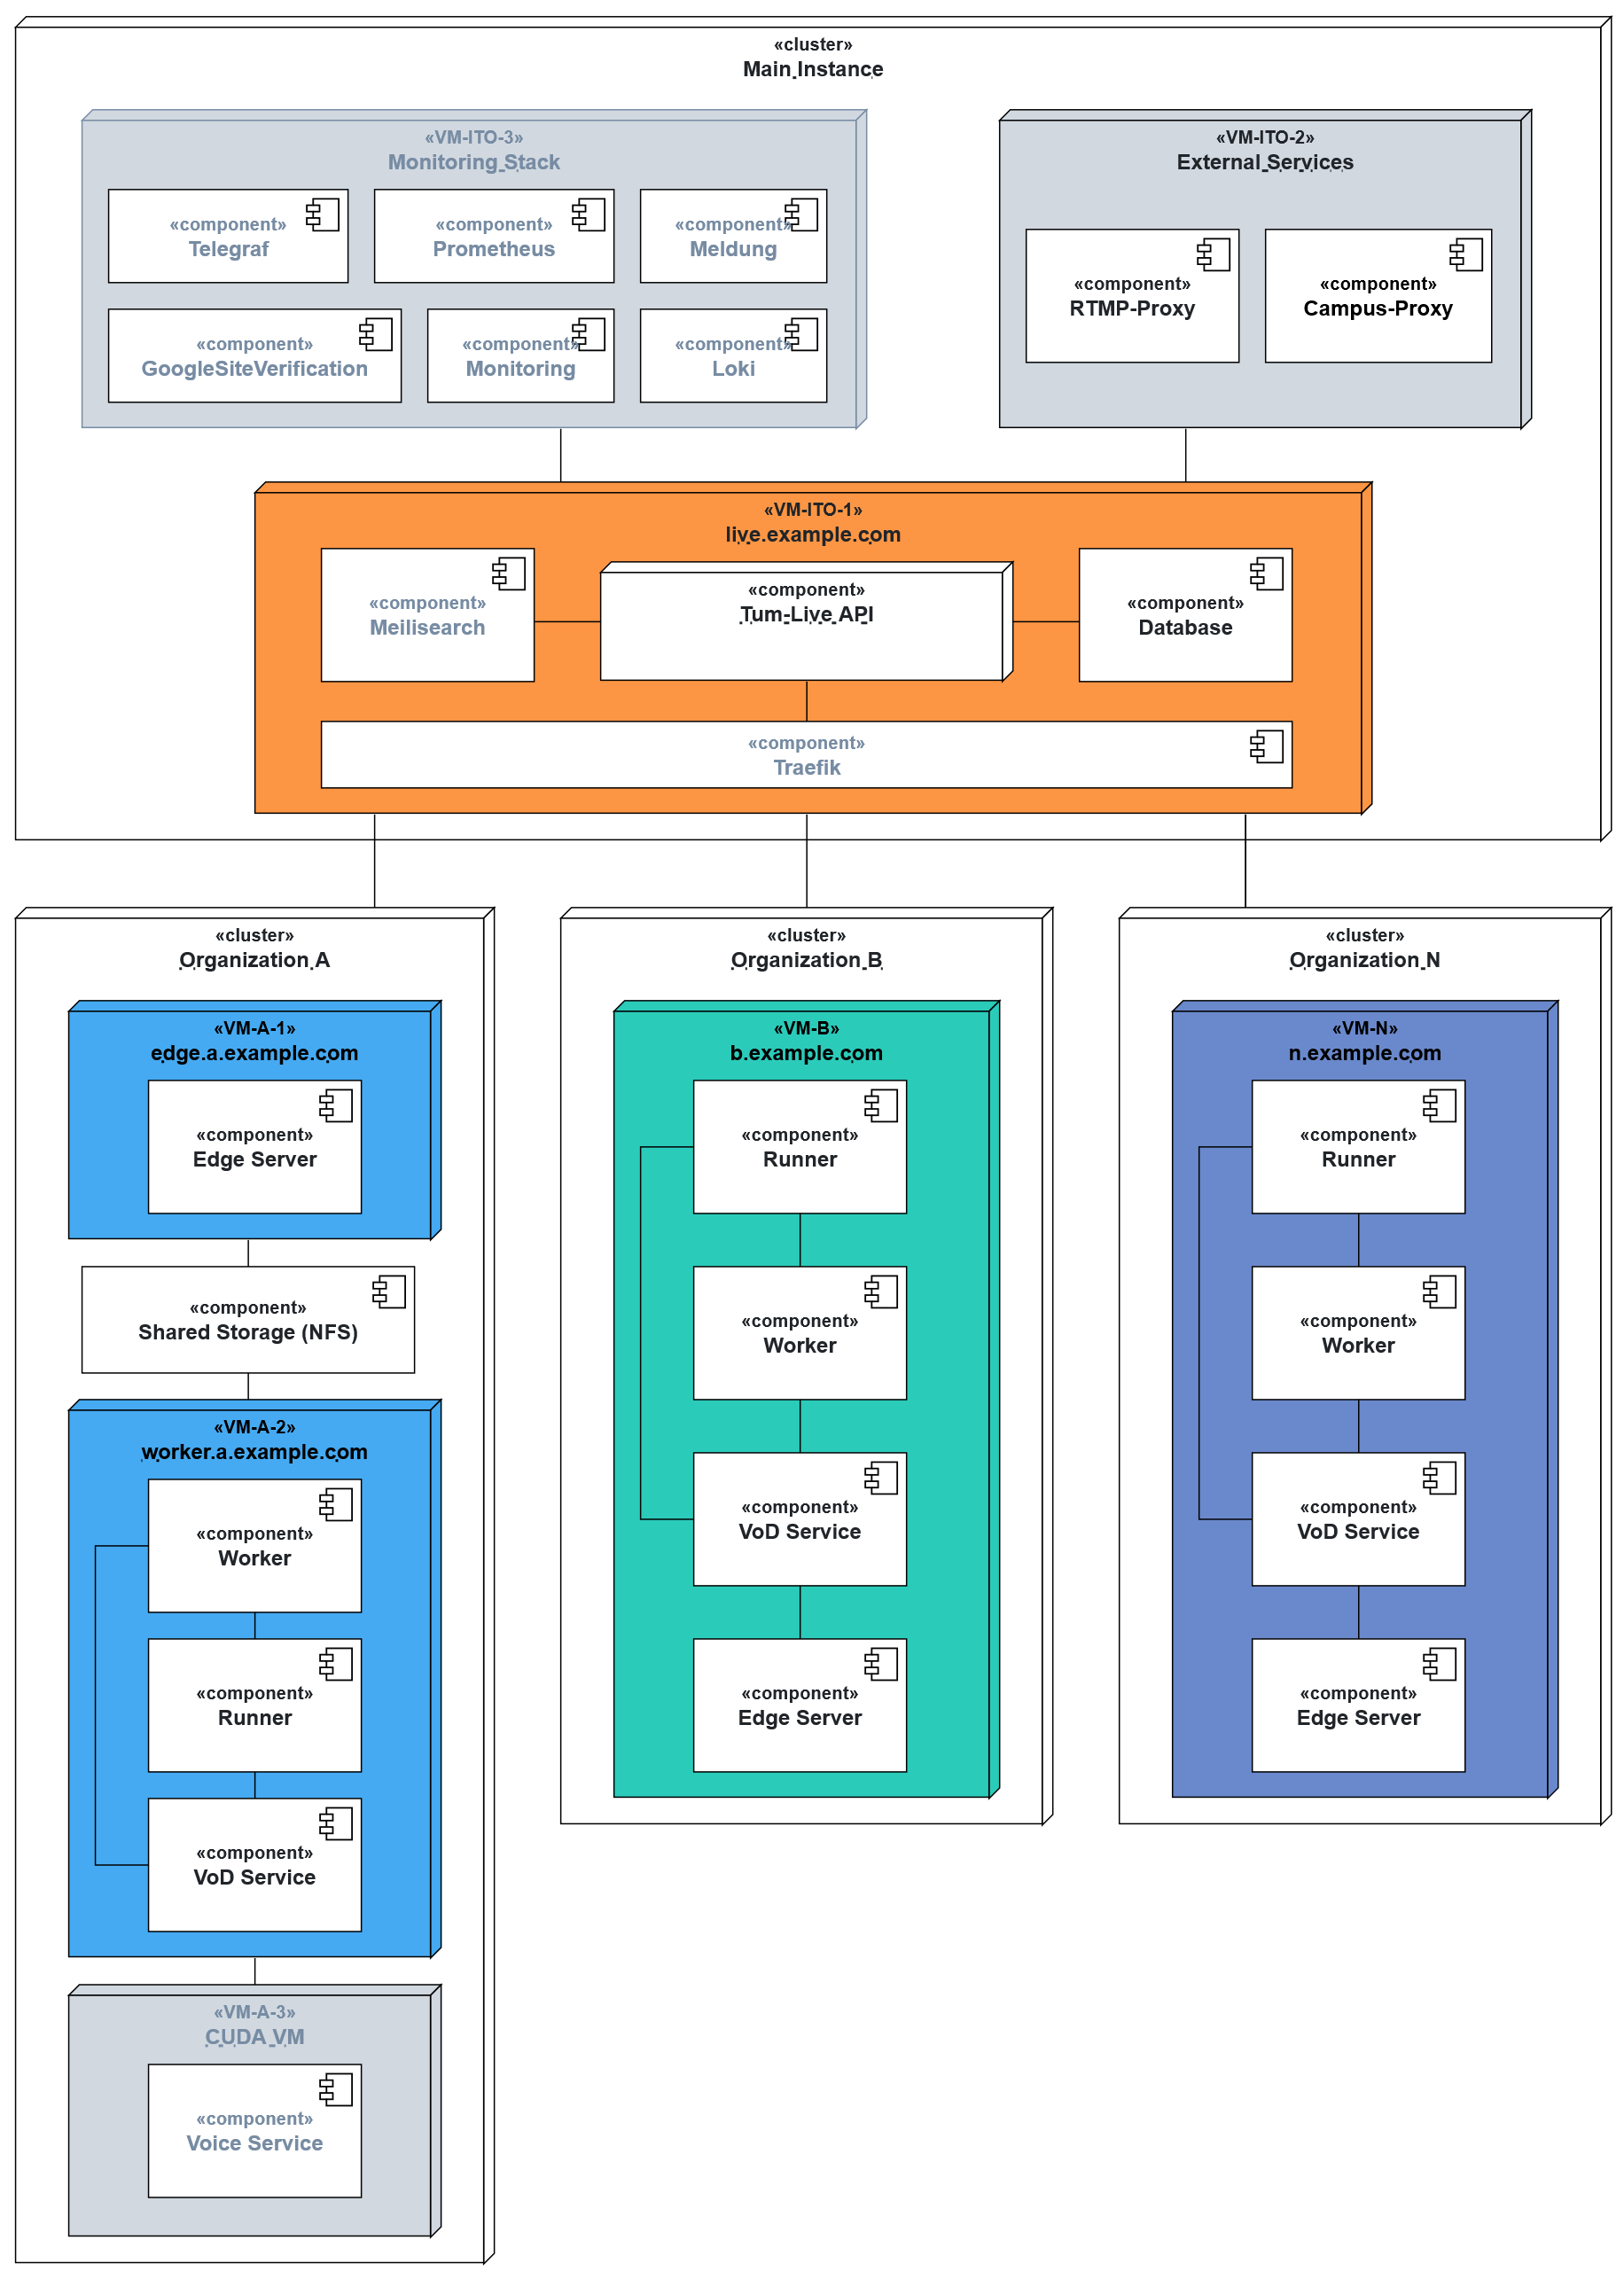
\includegraphics[width=400pt]{images/DeploymentDiagramNew.png}
    \caption[Target Deployment Diagram of TUM-Live]{Target Deployment Diagram of TUM-Live\footnotemark[5]}
    \label{fig:system-architecture}
\end{figure}

To distribute TUM-Live to different schools and universities, the subsystems and components responsible for processing and storing video data need to be distributed and hosted by each individual organization. 
The main TUM-Live \ac{API} instance however, will remain managed by the \ac{CIT} \ac{ITO} or \ac{TUM} so that users have a single point of access instead of having to switch instances when wanting to watch lectures of different schools.
To achieve this, each organization needs to host at least three components: the Worker component, the VOD Service component and an Edge Server. 
Each organization can decide how many resources it wants to allocate to each service depending on the expected load. The following minimum requirements are set:

\begin{itemize}
    \item At least 1 \ac{VM} as an Edge Server. This server serves the videos to the users. Throughput is important, so, to serve many users, more instances are needed.
    \item At least 1 Worker \ac{VM} to receive the stream and transcode the \ac{VOD}. On the same node, for every Worker a VOD Service needs to be deployed to expose a simple HTTP interface that accepts file uploads and packages them to a \ac{HLS} stream in a configured location. This stream may then be distributed by the Edge Server.
    \item Optionally, an organization can add additional \ac{VM}s for monitoring (\href{https://github.com/grafana/grafana}{Grafana}\footnote{\url{https://github.com/grafana/grafana}}, \href{https://github.com/prometheus/prometheus}{Prometheus}\footnote{\url{https://github.com/prometheus/prometheus}}, etc.) or for deploying services such as the Voice Service for subtitling live streams and \ac{VOD}s using the \href{https://github.com/openai/whisper}{Whisper LLM}\footnote{\url{https://github.com/openai/whisper}}.
\end{itemize}

\footnotetext[5]{In comparison to a \textit{System Architecture Model} (e.g., \autoref{fig:twitch-architecture}, \autoref{fig:youtube-system-design} or \autoref{fig:old-system-architecture}), a \textit{Deployment Diagram} shows a concrete instance of an abstract system architecture.}

\section{Delegated Administration of Resources}\label{section:rbac}

Given the proposed system (see \autoref{fig:system-architecture}), this section documents how this system has been implemented and what the current limitations and potential improvements of the main user system are. 

\subsection{Updating Architecture and Core API}

As explained before, with increasing demand, GoCast must be extended for university-wide lecture streaming. The solution to this are \textbf{organizations} that allow for delegated partial administration of resources.

The first step of implementing this structure was updating GoCast's role system. Previously, it contained four roles: \texttt{admin}, \texttt{lecturer}, \texttt{student}, \texttt{visitor}. While admins can manage the entire system (e.g., create and delete lectures and users, as well as perform maintenance tasks), lecturers can only manage their own or create new lectures and students only manage their own profiles and preferences. However, with the introduction of organizations, this is not sufficient, as each organization needs to have its own organization-scoped admins that can manage their organizations' resources without being able to interfere with other organizations. To do this, a new \texttt{maintainer} role has been introduced (see \autoref{fig:school-hierarchy}).
With this, an organization using GoCast is managed by a set of maintainers of this organization. A user with the \texttt{maintainer}-role can be the maintainer of multiple organizations and also has maintainer rights for all sub-organizations of his organizations.  
Maintainers also have some basic administrative functionality that is limited to their organizations' scope (e.g., create, update and delete courses and streams only for those organizations that are administered by that maintainer). 

\subsection{GoCast Organizations}

TUMOnline has a strict hierarchical structure for its organizations (one school has multiple departments; one department has multiple chairs; one chair has multiple courses ...).
%
% On a side node, TUMOnline has 7 organizations, 29 departments and 487 chairs.
While TUM-Live is mainly used by the TUM, in principle it does not need to differentiate between organizational types that strictly. Organizations are only relevant when it comes to distributing the live streams and recordings of a certain entity to that entity's resources (e.g., Workers and VOD Services). Hence, the introduction of GoCast's organizations which represent an entity responsible for processing data. In practice, this is most of the time a TUMOnline school, however, one can also create a GoCast organization for a department, chair or smaller organization which is subordinated to another organization, depending on the specific situation.

Here is an example to illustrate this in a more detailed way:
The TUMOnline "School of Management" (SOM) wants to start using TUM-Live. Hence, the SOM's IT team contacts the admins of TUM-Live who then create a new \textit{SOM organization} in TUM-Live and assign the SOM IT team as maintainers.
The subordinated "Chair of Financial Management and Capital Markets" (FA), however, has its own data center and wants to host its lectures with its own resources. In this case, either one of the SOM maintainers or the \ac{CIT} \ac{ITO} can create a new organization in TUM-Live as a sub-organization of the \textit{SOM organization} and accordingly assign new maintainers from the FA-team. Now, the FA-maintainers have full control over their sub-organization and can connect their own resources from their data center with TUM-Live, independently of the SOM.

% The idea is the following: To avoid one entity having to manage and process all streaming data for the entire university (or multiple universities), GoCast is distributed to multiple entities. Each entity (aka GoCast 'organization') has so-called maintainers (users with the maintainer user role) that are allowed to manage the organization's resources such as Workers, VOD Services, etc.


% One maintainer can maintain multiple organizations.
% The following organization-related actions are allowed by a maintainer of an organization:

%     Create, update or delete organization

%     Create new tokens for that organization (required to add new resources)

%     Manage organization's resources

%     Manage organization's maintainers




\section{Distributed Resources}

Now that the user role system had been updated, the next step was to find a solution to have the different resources, such as Workers connected to the main cluster of Workers independent of the other organizations' resources. However, at the same time, they should be able to process and distribute requests between each other regardless of the organization they are in. This section explains in detail how each subsystem works as part of the distributed GoCast system. 

\subsection{Workers and Runners}
To set up a distributed network of Workers, the first step was to update the system in such a way that Workers could be connected by an organization's maintainer to the main network of GoCast. To do this, an organization's maintainer can create a new organization-token, a \ac{JWT} that expires after seven hours and allows its owner to connect new resources for the organization. % (see \autoref{fig:school-token}).

% \begin{figure}[htpb]
%     \centering
%     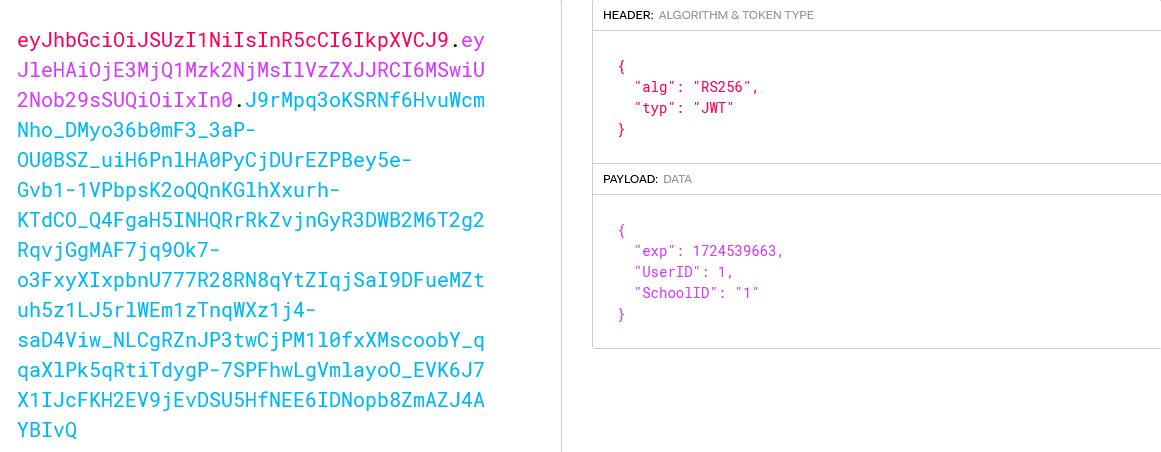
\includegraphics[width=390pt]{images/SchoolToken.png}
%     \caption[Example Organization Token]{Example Organization Token}\label{fig:school-token}
% \end{figure}

When a maintainer starts a new Worker, he can include this token in the container's environment (e.g., via a \texttt{docker-compose.yml} file or by passing it as an argument directly to Docker using \texttt{-e Token=<...>}). When starting up, the Worker sends a request to join the Worker pool of GoCast using the organization-token and additional data (e.g., host name, IP or FQDN address, \ac{VM} workload, etc.) and - if successful - receives a token without expiration which is then used to validate all subsequent requests from and to the Worker. Maintainers can then see and manage the current status of their registered resources in the Resource-Dashboard of GoCast (see \autoref{fig:resource-dashboard}).

\begin{figure}[htpb]
    \centering
    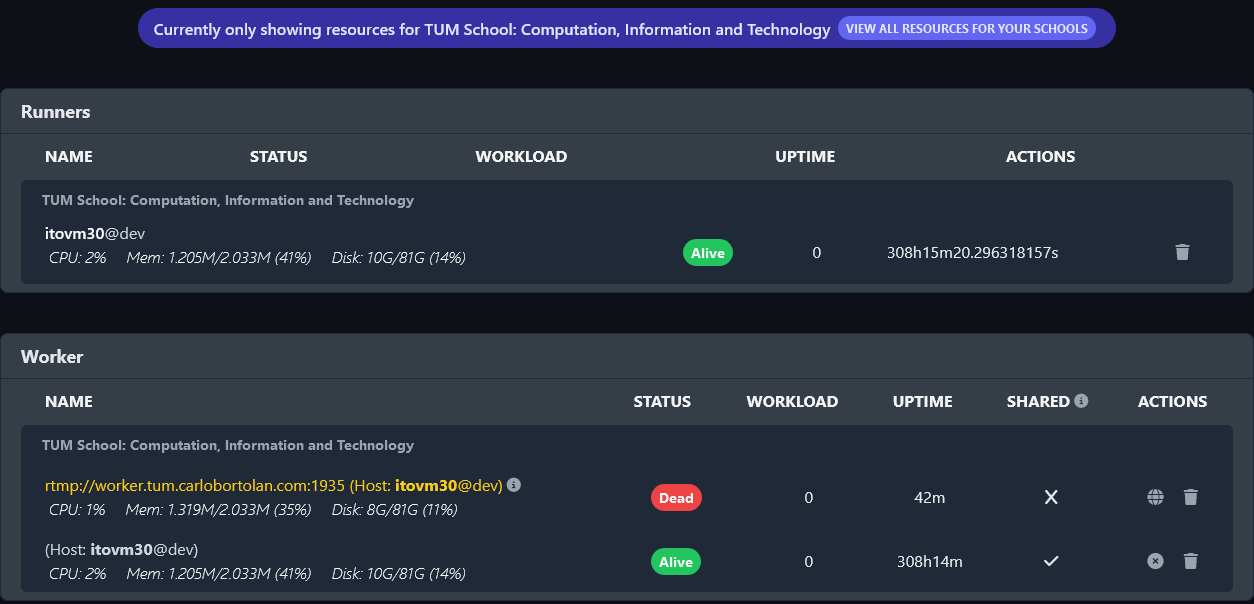
\includegraphics[width=390pt]{images/ResourceDashboard.png}
    \caption[Resources Dashboard]{Resources Dashboard}\label{fig:resource-dashboard}
\end{figure}

Now, whenever a new lecture is being received or uploaded, the main GoCast \ac{API} selects an available Worker for this organization and addresses it, given the hostname and IP address that the Worker has registered when first connecting to GoCast. For more details on how the distribution of tasks works, see \autoref{section:shared-resources}.

When the Worker receives such a request, it initiates the video transcoding process using \href{https://ffmpeg.org/}{FFmpeg}. The transcoding is performed based on the specific stream version\footnotemark[6]. 
The process is monitored in real-time, with progress being reported back to the GoCast system to ensure that any failed actions are retried with back-off strategies and that the final transcoded video meets the expected duration and quality standards.

\footnotetext[6]{\texttt{CAM} streams use a higher compression level (CRF 26) and lower priority (niceness 10), while \texttt{PRES} streams use lower compression (CRF 20) and higher priority (niceness 9), with specific tuning in FFmpeg for still images in presentations. \texttt{COMB} streams are assigned moderate compression (CRF 24) and the highest priority (niceness 8).}

\subsection{VOD Service and Edge Server}

Once the Worker has completed the transcoding process, the VOD Service starts detecting silent sections in the recordings so that the user will be able to skip these and jump directly to the start of the actual lecture. Then, it packages them into a \ac{HLS} stream and copies the packaged stream to the organization's recording storage.

To ensure easy access to these recordings, each organization also needs to have its own Edge Server set up. The VOD Service at each organization is responsible for managing the processing, packaging and storage of the recordings server-side, while the Edge Server is responsible for distributing the streams to the end users. This also has the advantage that each organization maintains full control over the storage of its streaming data.
Additionally, the Edge Server acts as a local cache for an organization's content. When students access recordings, the Edge Server distributes the content directly from the organization's storage, reducing the load on the organization's servers.

To allow for rapid post-processing and upload of \ac{VOD}s after a stream has ended, it is necessary that an organization has enough Workers to support the number of recorded lectures.
If an organization expects many concurrent viewers, it might need to consider having multiple Edge Servers running, as they have a limited bandwidth.
When network traffic to an Edge node exceeds the available bandwidth, the architecture might look like the example shown in \autoref{fig:edge-network}.

\begin{figure}[htpb]
    \centering
    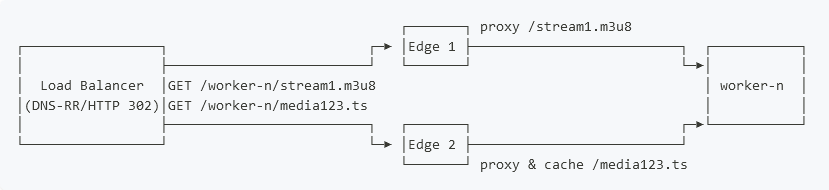
\includegraphics[width=\linewidth]{images/EdgeNetwork.png}
    \caption[Edge Server as Proxy and Cache Node]{Edge Server as Proxy and Cache Node}\label{fig:edge-network}
\end{figure}

% \subsection{Ingest Servers}
% TODO: How they are registered and distributed by the RTMP-Proxy
% \subsection{Voice Service}

\subsection{RTMP-Proxy}

\subsubsection{Limitaitons of GoCast's Self Streaming}

GoCast supports not just recordings from the lecture hall or manual uploads but also so-called self-streams. The idea behind self-streams is that any lecturer can go live at any given time and stream from his own device without having to be in the lecture hall. In past, to do this, a lecturer had to go open TUM-Live, go to one of his courses' page, select a lecture and copy a link (such as: \texttt{rtmp://worker.example.com/cs-123? secret=5caa9d6447564cb5822995888e224f9a}) together with a secret stream key into a streaming software like OBS Studio. With the introduction of the organization system, there are several reasons why this cannot work:

\begin{enumerate}
    \item The URL might change depending on the availability of Workers.
    \item Having to copy and paste a new URL every time a lecturer wants to start a stream can become annoying.
    \item For lecturers who teach at multiple organizations (e.g., a mathematics professor teaching lectures at the \ac{CIT} and at the School of Engineering and Design), managing different URLs for each organization would be inconvenient.
\end{enumerate}

\subsubsection{Proposed Solution and Data-Flow}

The solution for this is the RTMP-Proxy microservice. In a nutshell, the RTMP-Proxy acts as a router-like service that accepts all \ac{RTMP} self-stream requests and redirects them to an organization's Worker depending on the stream's course. With this, all a lecturer has to do is create a new personal token (see \autoref{fig:personal-token}) and copy the token together with the target URL of the RTMP-Proxy into a streaming software only once.
After this initial setup, the lecturer can go live whenever they want by simply using the pre-configured URL and token.

\begin{figure}[htpb]
    \centering
    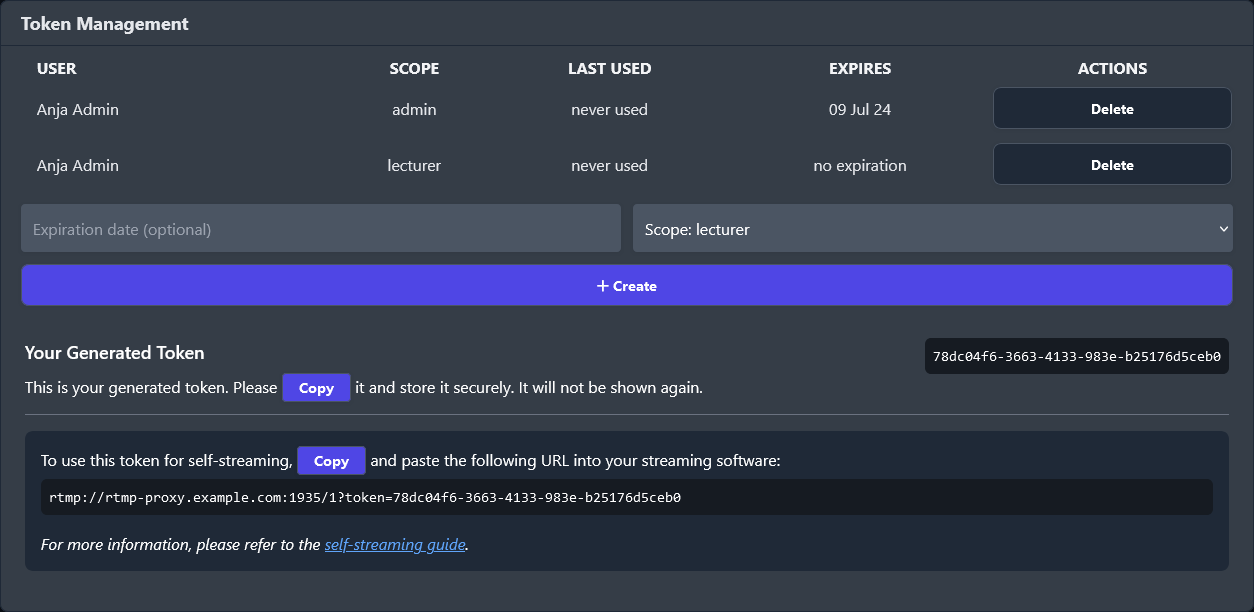
\includegraphics[width=\textwidth]{images/PersonalToken.png}
    \caption[Creation of Personal Token in TUM-Live and RTMP-Proxy URL]{Creation of Personal Token in TUM-Live and RTMP-Proxy URL}\label{fig:personal-token}
\end{figure}


The internal process of the RTMP-Proxy is as follows (see also \autoref{fig:rtmp-proxy}): 

\begin{enumerate}
    \item An incoming \ac{RTMP} request is received:\\
    \texttt{rtmp://proxy.example.com/live/<personal-token>}.
    \item The RTMP-Proxy sends a self-stream request to the main GoCast \ac{API} with the provided \texttt{personal-token}.
    \item The GoCast \ac{API} validates the \texttt{personal-token} and uses it to detect whether the lecturer has a scheduled lecture for the current time slot or a soon upcoming lecture and automatically starts the live stream with a waiting screen for viewers. Then it checks the stream's course's organization and returns the \ac{RTMP} URL of the ingest Worker currently available for that organization together with the course-slug and secret stream key for this stream: \\ 
    \texttt{rtmp://worker.example.com/<course-slug>?secret=<secret>/<secretKey>}.
    \item The RTMP-Proxy redirects the \ac{RTMP} request to the retrieved \ac{RTMP} URL.
    \item The organization's ingest Worker now receives the proxied \ac{RTMP} request as if it were sent directly to it by the lecturer's streaming software.
\end{enumerate}

\begin{figure}[htpb]
    \centering
    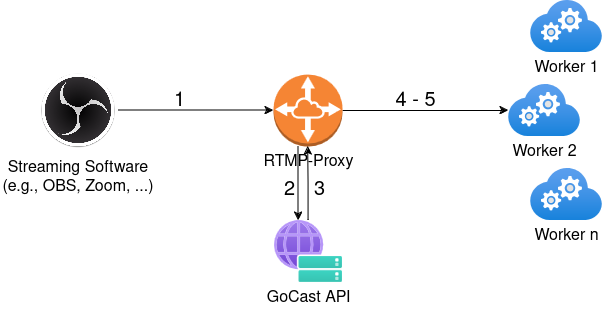
\includegraphics[width=300pt]{images/RtmpProxy.png}
    \caption[RTMP-Proxy Flow]{RTMP-Proxy Data Flow}\label{fig:rtmp-proxy}
\end{figure}

\subsubsection{Architectural Challenges and Limitations with RTMP}

Initially, for the prototype of the RTMP-Proxy the idea was to develop a microservice similar to the Edge Server or VOD Service written in Go that would redirect the \ac{RTMP} request (similar to an HTTP 302 redirect). However, after some testing, it quickly became obvious that Go does not yet have libraries to handle \ac{RTMP} requests with the necessary granularity. Hence, to proceed with this approach, it would require to use Go's native libraries to: 
\begin{itemize}
\item Handle the incoming \ac{RTMP} request
\item Perform a \ac{RTMP} handshake
\item Extract the user token from the \ac{RTMP} request
\item Find out the destination address
\item Establish a connection with the destination host
\item Streaming the video chunks directly to the destination address
\end{itemize}

\noindent This might work short term, but in the long term, it would lead to other problems with potential bugs, scalability issues, complex error handling and unknown security vulnerabilities if not properly maintained.

A better solution was to use the \href{https://github.com/arut/nginx-rtmp-module}{nginx-rtmp-module}\footnotemark[7]\footnotetext[7]{\url{https://github.com/arut/nginx-rtmp-module}} that extends Nginx to handle \ac{RTMP} streaming requests natively~\parencite{nginx_rtmp_module}. 
Now, whenever a stream request arrives at the proxy server, Nginx accepts the request and invokes a script that extracts the stream key (the personal token) and requests the actual destination URL from the GoCast \ac{API}. Upon receiving the destination URL, Nginx pushes the stream to the target server.

\subsubsection{Implementation Details: FFmpeg vs. OBS Compatibility}

During the testing phase, it was observed that at times streaming via FFmpeg worked perfectly fine, while some attempts using OBS failed:
\begin{itemize}
    \item \textbf{Encoding Mismatch}: FFmpeg explicitly specifies H.264 for video and AAC for audio. OBS, however, may set different default codecs. The target \ac{RTMP} server of the Worker required H.264 video and anything else would cause an error.
    \item \textbf{Bitrate Mismatch}: High bitrate settings in OBS were causing overloads, which led to connection issues with the target \ac{RTMP} server. Lowering the bitrate to 2500-4000 Kbps resolved the issue.
    \item \textbf{URL Composition}: The self-streaming URL used to call the proxy is structured like: \texttt{<protocol>://<host>:<port>/live/<stream\_key>}. OBS, however, requires the URL and stream key to be set separately (see \autoref{fig:obs-rtmp}).
\end{itemize}

\begin{figure}[htpb]
    \centering
    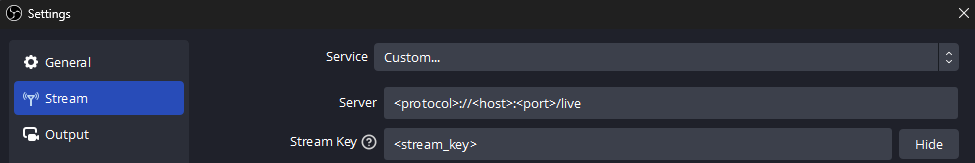
\includegraphics[width=\linewidth]{images/OBSRTMP.png}
    \caption[OBS Settings for Self-Streaming]{OBS Settings for Self-Streaming}\label{fig:obs-rtmp}
\end{figure}

This was later fixed by changing the settings in OBS and setting the video encoder to \texttt{x264} (H.264), the audio encoder to \texttt{AAC}, adjusting the bitrate to a more reasonable level and settings the keyframe interval to 2 seconds for better compatibility with the Nginx \ac{RTMP} server.

\subsubsection{Final Words on Scaling the RTMP-Proxy}

While the RTMP-Proxy is far from perfect, it is meant as a prototype of a possible solution to stream via \ac{RTMP} using OBS in a distributed network where the final target address of the stream request is unknown when making the request. As the RTMP-Proxy is independent of other services in the GoCast environment (besides the main \ac{API} to receive the destination URL), it can be scaled very easily by deploying multiple RTMP-Proxies and having, for example, a Round-robin DNS distribute the load accordingly.

\section{Shared Resources}\label{section:shared-resources}

This section explains different approaches for the allocation of resources in the GoCast network. The main focus is on the task distribution to the available Workers when receiving new video uploads or stream requests.

\subsection{Organization Hierarchy}
Before explaining how resources in the GoCast Network are dynamically allocated to different tasks, it is first important to explain in detail how an organization actually "owns" a certain resource such as a Worker. As described in \autoref{section:rbac}, organizations are structured in a hierarchical manner. One organization can have multiple sub-organizations, which can again have multiple sub-sub-organizations and so forth. When an organization has deployed its own resources, by default, they are accessible only by the organization itself and its sub-organizations. Using the example shown in \autoref{fig:school-hierarchy}, this would mean that if there is a lecture uploaded by \textit{Organization 1}, only public resources and the organization's own private resources are considered. For a lecture of \textit{Organization 2a}, all public resources, the organization's own private resources, as well as its parent organization's resources (and recursively so on) are considered. 

\begin{figure}[htpb]
    \centering
    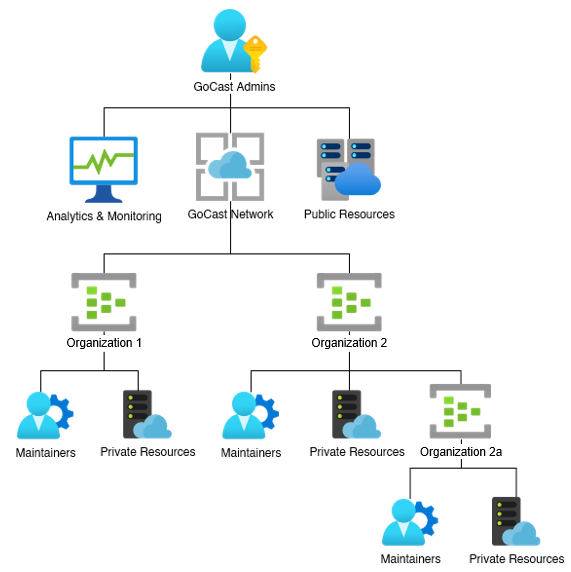
\includegraphics[width=350pt]{images/OrganizationHierarchy.png}
    \caption[Example Organization Hierarchy]{Example Organization Hierarchy}\label{fig:school-hierarchy}
\end{figure}

Additionally, for certain resources, for example, Workers, one can decide to set the \texttt{Shared} flag. When a resource has that flag enabled, it means that even though it is part of an organization (and hence by default only available for lectures of that organization or sub-organizations in that organization's hierarchy), it now becomes available to all organizations and shares its compute power with the entire network of organizations. To use the previous example, assuming that \textit{Organization 2a} has allowed to share its resources, when \textit{Organization 1} uploads a video or starts a stream, in addition to its own private resources and the public resources, it also considers the shared resource of \textit{Organization 2a}.

\subsection{Four Approaches for Task Distribution}

The following are four approaches considered for the decision algorithm behind the allocation of resources - especially of Workers - in the GoCast Network. The current implementation for the task distribution of Workers uses the second approach. For the Runners, it remains to be seen which approach will be chosen - most likely a combination of the second and third approaches. 

% \begin{enumerate}
    % \item \textbf{Randomized Allocation:}  
\subsubsection{1. Randomized Allocation}
     Tasks are assigned to available resources randomly. This method is simple and helps to distribute tasks across resources in an unbiased manner. However, it only considers an organization's own and public resources, ignoring the hierarchical structure of organizations or resource workloads. Randomized allocation can be effective if resource capabilities were relatively uniform, but it would most likely lead to inefficiencies if the networks got more complex.

    \begin{figure}[htpb]
      \begin{tabular}{c}
      \ \small \begin{lstlisting}[language=SQL]
        -- 1. Randomized allocation example query
        SELECT *
        FROM workers 
        WHERE shared = TRUE OR org_id = ?
        ORDER BY RANDOM()
        LIMIT 1;
        \end{lstlisting}
      \end{tabular}
      \label{fig:randomized-allocation}
    \end{figure}
    
    % \item \textbf{Recursive Organization-Based Allocation:}  
\subsubsection{2. Recursive Organization-Based Allocation}
    When a task is started, the system recursively checks for available resources, starting from the organization's own private resources and moving up the hierarchy to include parent organizations and shared resources as described in the previous subsection. With this approach, each task is allocated to the most appropriate resource, improving resource utilization across the GoCast system by allowing sub-organizations to benefit from the resources of their parent organizations while respecting the resource ownership of each organization. One could implement different optimizations, such as prioritizing one's own resources before shared resources or limiting how many levels the query should follow the parent-child relationship upwards. Also, one organization might not want to use resources shared by other organizations and, therefore, include only resources from its own organization's hierarchy. The code snippet below is an example of how a recursive query might look to find all available Workers in an organization's hierarchy, including shared Workers.   

    \begin{figure}[htpb]
      \begin{tabular}{c}
      \ \small \begin{lstlisting}[language=SQL]
        -- 2. Recursive organization-based allocation example query
        -- First, create a recursive query to follow the parent-child hierarchy upward
        WITH RECURSIVE org_hierarchy AS (
            SELECT id, parent_id FROM orgs WHERE id = ?
            UNION ALL
            SELECT o.id, o.parent_id FROM orgs o
            INNER JOIN org_hierarchy oh ON o.id = oh.parent_id 
        ) 
        -- Then, select all Workers that are in the hierarchy or shared
        SELECT w.* FROM workers w
        LEFT JOIN org_hierarchy oh ON oh.id = w.org_id
        WHERE oh.id IS NOT NULL OR w.shared = true;
        \end{lstlisting}
      \end{tabular}
      \label{fig:recursive-allocation}
    \end{figure}

    % \item \textbf{Priority-Based Allocation:}  
\subsubsection{3. Priority-Based Allocation}
    Tasks are assigned to Workers based on a dynamically adjusted priority queue. The tasks would be prioritized based on factors such as viewer count, failure rate, \ac{VM} workload or the type of content being processed. For example, live streaming tasks could be given a higher priority over \ac{VOD} uploads and hence be processed by a Worker that runs on a more powerful \ac{VM}. This approach would assign critical tasks (e.g., live streaming) first and re-schedule less urgent tasks (e.g., \ac{VOD} uploads or thumbnail generation) for later. The example below shows one possible implementation of the selection process, assuming that the \texttt{taskQueue} contains tasks sorted by priority. 

    \begin{figure}[htpb]
      \begin{tabular}{c}
      \ \small \begin{lstlisting}[language=Java]
        // 3. Priority-based allocation pseudocode
        function processTaskQueue(taskQueue) {
            while not taskQueue.isEmpty() {
                task = taskQueue.dequeue() // Get task with highest priority
                worker := getNextAvailableWorker() // Find available Worker
                if worker != nil {
                    worker.assignTask(task)
                } else {
                    taskQueue.enqueue(task) // Requeue task if no Workers are available
                }
            }
        }
        \end{lstlisting}
      \end{tabular}
      \label{fig:priority-based-allocation}
    \end{figure}

\subsubsection{4. Linear Programming Optimization Approach}

By solving a \ac{LP}, the tasks can be distributed evenly among Workers, minimizing the maximum load on any single worker and reducing bottlenecks.

\begin{enumerate}
    \item \textbf{Variables and Parameters}

Let:
\begin{itemize}
    \item \( n \) be the number of tasks.
    \item \( m \) be the number of Workers.
    \item \( t_i \) be the processing time of task \( i \) estimated using past averages or heuristics based, for example, on the scheduled stream's duration.
    \item \( x_{ij} \) be a binary decision variable, where \( x_{ij} = 1 \) if task \( i \) is assigned to Worker \( j \) and \( x_{ij} = 0 \) otherwise.
    \item \( L_j \) be the total workload on Worker \( j \), calculated as \( L_j = \sum_{i=1}^{n} t_i \cdot x_{ij} \).
    % \item \( L_{\text{max}} \) be the maximum load across all Workers, defined as \( L_{\text{max}} = \max_{j=1}^{m} L_j \).
\end{itemize}

\item \textbf{Objective Function}

The goal is to minimize \( L_{\mathrm{max}} \) across all Workers:
\begin{equation}
\operatorname{Minimize\ } L_{\text{max}}
\end{equation}

\item \textbf{Constraints}

The \ac{LP} is subject to the following constraints:

\begin{enumerate}
    \item \textbf{Task Assignment:} Each task \( i \) must be assigned to exactly one Worker:
    \begin{equation}
    \sum_{j=1}^{m} x_{ij} = 1 \quad \forall i = 1, \dots, n
    \end{equation}

    \item \textbf{Load Calculation:} The workload of each Worker \( j \) is the sum of the processing times of the tasks assigned to that Worker:
    \begin{equation}
    L_j = \sum_{i=1}^{n} t_i \cdot x_{ij} \quad \forall j = 1, \dots, m
    \end{equation}

    \item \textbf{Bounding the Maximum Load:} The workload on each Worker must be less than or equal to the maximum load \( L_{\text{max}} \):
    \begin{equation}
    L_j \leq L_{\text{max}} \quad \forall j = 1, \dots, m
    \end{equation}
    
    \item \textbf{Binary Variables:} The assignment variables \( x_{ij} \) are binary:
    \begin{equation}
    x_{ij} \in \{0, 1\} \quad \forall i = 1, \dots, n \quad \text{and} \quad \forall j = 1, \dots, m
    \end{equation}
\end{enumerate}

\item \textbf{Linear Programming Formulation:}

Given the objective function and the constraints, the solution to the \ac{LP} can be formulated as:
\begin{align}
\text{Minimize} \quad & L_{\text{max}} \\
\text{subject to} \quad & \sum_{j=1}^{m} x_{ij} = 1 \quad \forall i = 1, \dots, n \\
& L_j = \sum_{i=1}^{n} t_i \cdot x_{ij} \quad \forall j = 1, \dots, m \\
& L_j \leq L_{\text{max}} \quad \forall j = 1, \dots, m \\
& x_{ij} \in \{0, 1\} \quad \forall i = 1, \dots, n \quad \text{and} \quad \forall j = 1, \dots, m
\end{align}
\item \textbf{Example Implementation:} 

    \begin{figure}[htpb]
      \begin{tabular}{c}
      \ \small \begin{lstlisting}[language=Python]
        # Using Gurobi as an example - any other solver also works
        from gurobipy import Model, GRB, quicksum
        model = Model("Minimize_Max_Load")
        
        # Decision variables: x[i, j] = 1 if task i is assigned to Worker j, 0 otherwise
        x = model.addVars(n, m, vtype=GRB.BINARY, name="x")
        
        # Variable for maximum load across all Workers
        L_max = model.addVar(vtype=GRB.CONTINUOUS, name="L_max")
        
        # Objective: Minimize the maximum load L_max
        model.setObjective(L_max, GRB.MINIMIZE)
        
        # Constraint 3.a) Each task is assigned to exactly one Worker
        for i in range(n):
            model.addConstr(
                quicksum(x[i, j] for j in range(m)) == 1, name=f"Task_Assignment_{i}")
        
        # Constraint 3.b) and 3.c) Load on each Worker does not exceed L_max
        for j in range(m):
            model.addConstr(
                quicksum(t[i] * x[i, j] for i in range(n)) <= L_max, 
                name=f"Worker_Load_{j}")
        
        # Run the model
        model.optimize()
        \end{lstlisting}
      \end{tabular}
      \label{fig:lp-optimization}
    \end{figure}

\end{enumerate}
